\documentclass[border=5pt]{standalone}
\usepackage{tikz}

\begin{document}
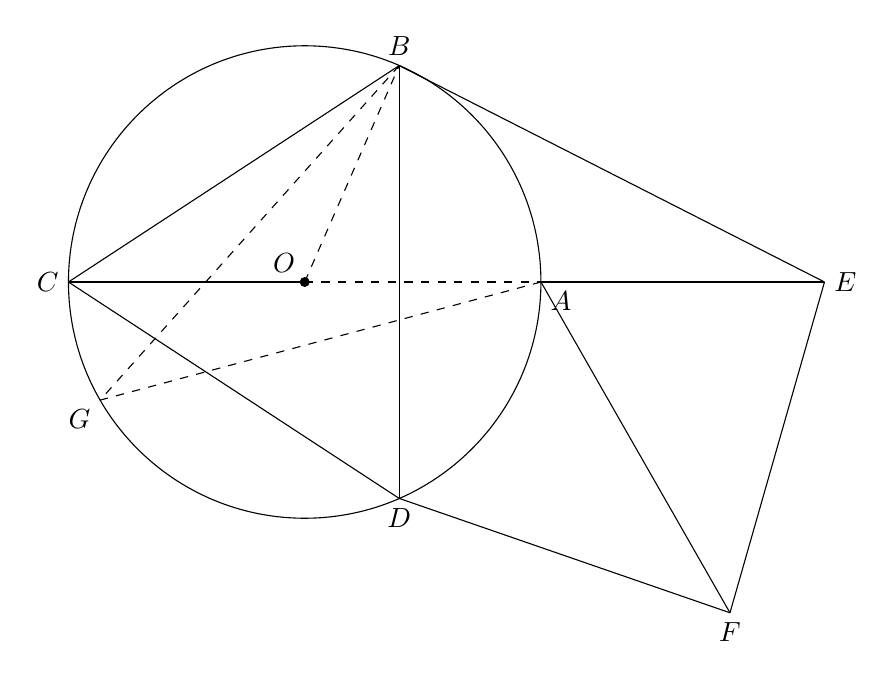
\begin{tikzpicture}[scale=1.2]
    % Define coordinates
    \coordinate (O) at (0,0);
    \coordinate (C) at (-2.5, 0);
    \coordinate (A) at (2.5, 0);
    \coordinate (E) at (5.5, 0);
    
    % B and D. x=1, R=2.5 -> y=sqrt(6.25-1)=2.29
    \coordinate (B) at (1, 2.29);
    \coordinate (D) at (1, -2.29);
    
    % G. Angle 210 degrees.
    \coordinate (G) at ({2.5*cos(210)}, {2.5*sin(210)});
    
    % F.
    \coordinate (F) at (4.5, -3.5);

    % Circle
    \draw (O) circle (2.5);
    
    % Solid Lines
    \draw (C) -- (B);
    \draw (C) -- (D);
    \draw (B) -- (D); 
    \draw (B) -- (E);
    \draw (A) -- (E); 
    \draw (C) -- (O); 
    
    \draw (A) -- (F);
    \draw (E) -- (F);
    \draw (D) -- (F);
    
    % Dashed Lines
    \draw[dashed] (O) -- (B);
    \draw[dashed] (A) -- (G);
    \draw[dashed] (B) -- (G);
    \draw[dashed] (O) -- (A); % Modified AO to dashed
    
    % Labels
    \fill (O) circle (1.5pt);
    \node[above left] at (O) {$O$};
    \node[left] at (C) {$C$};
    \node[below right] at (A) {$A$};
    \node[above] at (B) {$B$};
    \node[below] at (D) {$D$};
    \node[right] at (E) {$E$};
    \node[below] at (F) {$F$};
    \node[below left] at (G) {$G$};
\end{tikzpicture}
\end{document}
